% Chapter 1

\chapter{Introduction} % Main chapter title
\thispagestyle{nohead}
\label{Intro} % For referencing the chapter elsewhere, use \ref{Intro} 

%----------------------------------------------------------------------------------------

% Define some commands to keep the formatting separated from the content 
\newcommand{\keyword}[1]{\textbf{#1}}
\newcommand{\tabhead}[1]{\textbf{#1}}
\newcommand{\code}[1]{\texttt{#1}}
\newcommand{\file}[1]{\texttt{\bfseries#1}}
\newcommand{\option}[1]{\texttt{\itshape#1}}
%----------------------------------------------------------------------------------------
As software development projects grow in size and budget, so does the cost, time, and complexity associated with fixing the problems that inevitably arise.
As an example of a particularly expensive error, in 1996 the Ariane 5 rocket exploded soon after launch due to a numerical conversion error: costing \$350 million \cite{Charette:2005:WSF:2241236.2242319}. 
Software engineering (SE) as a field has introduced concepts, models and techniques intended to combat such problems:
\begin{itemize}
	\item Software process models (e.g. agile development).
	\item Specifications for the abstraction of systems (e.g. the Unified Modelling Language \cite{UML}).
	\item Methodologies to ensure the safety of a system (e.g. unit testing).
\end{itemize}
This thesis is based on tool support for software verification (SV). 
In terms of the categories listed above, SV is concerned with the safety of a system.
In contrast to software testing which ensures a program behaves as \textit{expected} for a given set of inputs, SV ensures the programs behave as \text{specified} for \textit{all possible} inputs.
SV tools achieve this through logical reasoning based on formal specifications.
The consequences for the safety and reliability of complex software systems can be impressive. 
One SV tool, Atelier B, was used to verify the correctness of software operating the (driver-less) Line 14 of the Paris m\'etro \cite{Atelier-B}. 
 
The three examples of software engineering techniques above have benefited from excellent tool support and have been widely adopted by software developers.      
Software verification systems, however, often require specialised knowledge and suffer from a lack of integrated tool support \cite{Alglave2011}.     
The automation of processes requiring domain-specific knowledge can be an important technique to encourage the adoption of new software engineering practices.
This thesis presents a tool to automate one such process for the \textsf{Why3} \cite{why:shephard} software verification system. 
By providing a layer of abstraction to the \textsf{Why3} back-end architecture, we hope to make the system more approachable for software engineers without \textit{specific knowledge} of the tools interfaced by the \textsf{Why3} system. 
 
\section{Introducing \textsf{Why3}}
%Software Verification Systems as Composed of Modular Components
In general, software verification systems can be viewed as being composed of the following components: 

\begin{enumerate}
	\item A developer-facing front-end.
	\item An intermediate logic language (IVL).
	\item A back-end to solve proof obligations (POs).
\end{enumerate}

This section will discuss \textsf{Why3}'s modular and extensible approach to these three components compared to other SV systems. 
%In general, the \textsf{Why3}system is more modular and extensible than the other SV systems referenced in this section (and again in the Literature Review Sec. \ref{sec:lrsv}). 
%The components of which tend to be more tightly-integrated.

\subsection{A developer-facing front-end} 

Usually this component takes the form of either a special-purpose programming language (such as Dafny \cite{Dafny}) or the modification of an existing language such as Java (the Java Modelling Language (JML) \cite{JML}) or C\# (via Spec\# \cite{spec}). 
In either case, the language must support verification constructs such as data invariants, pre- and post- conditions.
%The front-end should allow for high-level constructs and modularisation:   
%to support verification constructs and program specification features. This second approach is used by  and  which is based on C\#. 

The WhyML \cite{why:polymorphic} programming language is based on Standard \texttt{ML}. 
Polymorphic types, a module system and a large library of verified data structures make the language approachable and familiar to software engineers.
WhyML programs are natively supported by the \textsf{Why3} integrated development environment (IDE). 

There are a number of projects building alternative front-ends for the \textsf{Why3} system. 
The Jessie plugin \cite{Jessie:manual} provides deductive verification capabilities for C programs and the SPARK 2014 \cite{spark} environment supports the verification of Ada programs through the \textsf{Why3} system. 
Both these projects translate POs directly into the Why IVL.	
	
\subsection{An intermediate logic language} 

Assertions about a program's properties are formally translated to a lower-level logic language.
The IVL typically supports axiomatisation of the program's constraints and other common concepts such as linear arithmetic, arrays etc. A number of proof obligations (POs) are generated by the translation process. 
The POs must be satisfied in order for the program to be verified.
The Boogie language \cite{Boogie} is the IVL used by both the Dafny and Spec\# verification systems.

The logic of \textsf{Why3}'s IVL is an extension of first-order logic which supports polymorphic types, algebraic data types, quantifiers, recursive and inductive predicate definitions.
As it is the front-end to a wide range of automatic and interactive theorem proving tools, the Why IVL is designed to be expressive and efficient.
The major benefit to using \textsf{Why3}'s IVL is the capability to send the generated POs to a number of theorem-proving tools at the back-end.
This capability, and the flexibility of the language's logic, has led to a growing number of projects translating the output from Atelier-B \cite{atelierB2w, rodinplugin} and Boogie \cite{b2w} to the Why logic language.  

\subsection{PO-discharging back-end} 

In order for each PO to be proven satisfiable or otherwise, they must be sent to a special-purpose program which implements the appropriate decision procedures for the logical theories referenced by the IVL. This back-end component may be a Satisfiability (SAT) solver; in which case, all constraints are translated into a boolean formula of propositional logic with a number of unknown values. The solver's task is to prove whether there is some assignment of these variables which satisfies the formula. 
	
More often, however, a Satisfiability Modulo Theories (SMT) solver is used for SV system back-ends. SMT solvers extend SAT solvers by implementing decision procedures for a number of logical theories. A specific algorithm has been developed to decide problems using arrays or linear arithmetic, for example. The combination of these algorithms allow SMT solvers to prove formul\ae~using a more expressive range of logical theories than propositional logic. Z3 \cite{Z3} is an example of a popular and powerful SMT solver. It is used to discharge POs generated by the Boogie, Spec\# and Dafny tools. 

This component is where \textsf{Why3} differs most from other SV systems.
It implements a modular architecture based on drivers.
Using a specific driver file, \textsf{Why3} writes the input format for each supported automatic theorem prover (ATP) such as MetiTarski \cite{Akbarpour2008} and Gappa \cite{gappa} (which specialise in solving numerical problems), SMT solver (the SMT solvers supported by \textsf{Why3} will be introduced later in the thesis) and interactive theorem prover (ITP) (sometimes called a \textit{proof assistant}) such as Coq \cite{Coq} and Isabelle \cite{Isabelle}.
This driver file lists the transformations that must take place (e.g. remove polymorphism or inductive predicates) in order for \textsf{Why3}'s logic to conform to that of the theorem proving tool.

%\subsection{An overview of various \textsc{SMT} solvers and their capabilities}
\section{Thesis Statement}

Having such a range of ATP, SMT and ITP tools supported by a single IVL is a welcome development.
Increased operability in the SV domain lets users utilise the most appropriate tool for their specific task.
However, time can be wasted if the wrong tool is consistently chosen. 
For example, Z3 has a unique and effective approach to reasoning about quantifiers, while the Alt-Ergo \cite{AltErgo} SMT solver produces excellent results for POs containing polymorphic types.

By choosing the most appropriate SMT solvers, more POs can be proven and safer software can be developed.
Without knowing which SMT solver \textit{is} the most appropriate, however, this choice is essentially a random one.
We present a method to automate the choice of SMT solver for any given proof obligation.
The resultant tool, which we have named \where, is a ``portfolio solver'': it is a portfolio of solving algorithms consisting of several SMT solvers.
It attempts to choose the most appropriate of these solvers based on static metrics derived from each PO's syntactic features.  
Our project's thesis statement: 
 
\begin{quote}
	\textit{The use of portfolio-solving techniques results in the efficient and \nobreakdash automatic allocation of SMT resources which prove a maximal number of \nobreakdash software verification proof conditions.}
\end{quote}

This work is intended for use by the non-expert developer performing SV as part of an enlightened software development process.
This user has no specific knowledge of the internal implementation of individual SMT solvers nor of their relative strengths and weaknesses. 
They may not even know the particular characteristics of the PO they are trying to prove (hidden as they may be through the use of a front-end specification language).
A PO may be characterised by its use of universal quantifiers or non-linear arithmetic, for example.

We limit this work to the use of SMT solvers in order to make valid comparisons about each tool's suitability for SV-specific tasks.
As we shall discuss in Sec. \ref{sub:lrsvmmbench}, the lack of a standard input format for SV systems makes their comparative evaluation difficult.
The opportunity to make such an evaluation is a secondary aim for this project.

\section{Contributions}
The main contributions of this work are:
\begin{enumerate}
	\item The design  and implementation of a portfolio solver, \where, which uses supervised machine learning to predict the best solver to use based on metrics collected from goals.
	\item The integration of \where~into the user's existing \textsf{Why3} work-flow by imitating the behaviour of an orthodox SMT solver.
	\item A set of metrics to characterise \textsf{Why3} goal formul\ae.
	\item Statistics on the performance of eight SMT solvers using a dataset of 1048 \textsf{Why3} goals.
	\item An evaluation of six machine learning algorithms' performance when predicting the most appropriate SMT solvers, given a \textsf{Why3} PO.  
	
\end{enumerate}

\section{Organisation of this thesis}

\begin{figure}
	\centering
	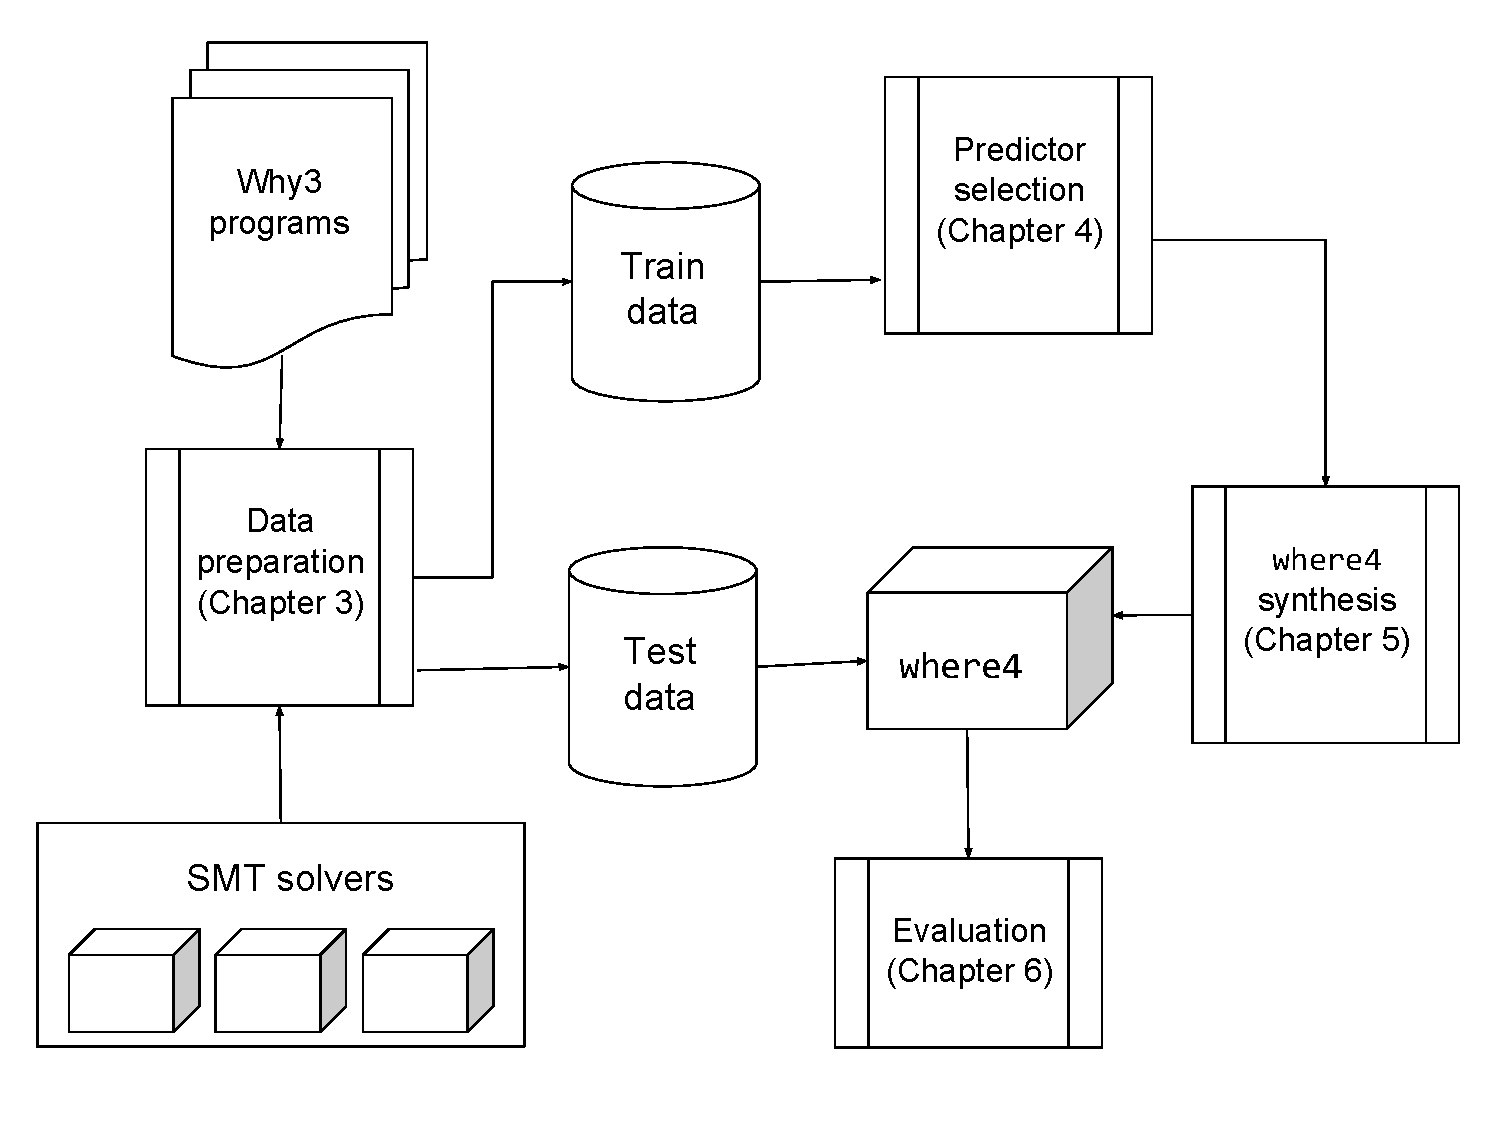
\includegraphics[width=0.9\linewidth]{Figures/intoduction}
	\caption{Overview of the \where~project and this thesis's structure}
	\label{fig:introduction}
\end{figure}

We view this research as being situated at the intersection of three broad research areas within computer science: software verification, the measurement of software through metrics, and machine learning (ML). 
Chapter \ref{LitReview}'s literature review reflects these themes and focusses particularly on their intersection.  

The organisation of the rest of this thesis, and the associated data / artefacts produced during the development of \where, is illustrated in Fig. \ref{fig:introduction}. 
Chapter \ref{Experimental} discusses the choices we made regarding the experimental setup of our empirical study. 
These choices include the dataset of \textsf{Why3} POs and the portfolio's individual SMT solvers.
The process to choose and extract independent and dependent variables for the machine learning task is also described in this chapter.
Chapter \ref{Prediction} contains a discussion of the chosen solvers' performance on the dataset. 
A number of options considered for the prediction task and an evaluation of several ML algorithms' suitability for this task is contained in this chapter.

\sloppypar
Chapter \ref{Implementation} describes our implementation of the chosen model using \textsf{Why3}'s OCaml API.
The encoding of \where's ML model into OCaml data structures is discussed in this chapter.
Chapter \ref{Evaluation} defines three Evaluation Questions designed to assess the final \where~tool's performance, usability and practicality.
We evaluate \where~with reference to these questions.
Chapter \ref{Conclusion} concludes this thesis by reflecting on the contributions of our work and suggesting some future directions for this project.



